\begin{enunciado}
 Si graficamos las probabilidades de aceptaci\'on de $H_0$ que corresponden a diversas alternativas para $\mu$ (incluido el valor especificado por $H_0$) y conectamos todos los puntos mediante una curva suave, obtenemos la \textbf{curva caracter\'{\i}stica de operaci\'on} del criterio de prueba o, simplemente, curva \textit{CO}. Observe que la probabilidad de aceptaci\'on de $H_0$ cuando es verdadera es simplemente $1 - \alpha$. Las curvas caracter\'{\i}sticas de operaci\'on se utilizan ampliamente en aplicaciones industriales para brindar una muestra visual de los m\'eritos del criterio de prueba. Con referencia al ejercicio 10.15, encuentre las probabilidades de aceptaci\'on de $H_0$ para los siguientes $9$ valores de $\mu$ y grafique la curva \textit{CO}: $184$, $188$, $192$, $196$, $200$, $204$, $208$, $212$ y $216$.
\end{enunciado}

\begin{solucion}
 Usando los t\'erminos del ejercicio 10.15, se tiene lo siguiente:
 \begin{itemize}
  \item $X \sim n(\mu, \sigma)$.
  \item $\overline{X} \sim n\left( \mu, \sigma/\sqrt{n} \right)$.
  \item $n = 9$.
  \item $\sigma = 15$.
  \item $\sigma_{\overline{X}} = 15/\sqrt{9} = 15/3 = 5$.
  \item $x_{\text{inf}} = 191$ y $x_{\text{sup}} = 209$.
 \end{itemize}
 Antes de comenzar, n\'otese lo siguiente: los valores cr\'{\i}ticos inferior y superior son de la forma $200-k$ y $200+k$, con $k = 9$, mientras que si $\mu_1 = 200 - r$ y $\mu_2 = 200 + r$, para alg\'un valor $r$ no negativo, entonces, debido a la simetr\'{\i}a de la normalidad, se tiene lo siguiente:
 \begin{eqnarray*}
  P(\left. \text{Aceptaci\'on de } H_0 \right| \mu =\mu_1 ) & = & P\left( \left. 200 - k < \overline{X} < 200 + k \right| \mu_1 = 200 - r \right) \\
  & = & P\left( \frac{(200-k) - (200-r)}{5} < Z < \frac{(200+k) - (200-r)}{5} \right) \\
  & = & P\left( \frac{r-k}{5} < Z < \frac{r + k}{5} \right) \\
  & = & P\left( Z < \frac{r+k}{5} \right) - P\left( Z \leq \frac{r - k}{5} \right) \\
  & = & P\left( Z > -\frac{r+k}{5} \right) - P\left( Z \geq -\frac{r-k}{5} \right) \\
  & = & \left[ 1 - P\left( Z \leq \frac{-r-k}{5} \right) \right] - \left[ 1 - P\left( Z < \frac{-r+k}{5} \right) \right] \\
  & = & P\left( Z < \frac{-r+k}{5} \right) - P\left( Z \leq \frac{-r-k}{5} \right) \\
  & = & P\left( \frac{-r-k}{5} < Z < \frac{-r+k}{5} \right) \\
  & = & P\left( \frac{(200-k)-(200+r)}{5} < Z < \frac{(200+k)-(200+r)}{5} \right) \\
  & = & P\left( \left. 200-k < \overline{X} < 200+k \right| \mu_2 = 200+r \right) \\
  & = & P(\text{Aceptaci\'on de } H_0 | \mu = \mu_2)
 \end{eqnarray*}
 Por lo tanto, la probabilidad de aceptaci\'on de $H_0$ son iguales entre las parejas $\mu = 184$ y $\mu = 216$, $\mu = 188$ y $\mu = 212$, $\mu = 192$ y $\mu = 208$, y, $\mu = 196$ y $\mu = 204$.
 \par 
 Entonces, bajo el supuesto
 \begin{itemize}
  \item $\mu = 184$
 \end{itemize}
 la probabilidad de aceptaci\'on de $H_0$ se aproxima con las tablas A.3 como sigue:
 \begin{eqnarray*}
  P\left(191 < \overline{X} < 209 \right) & = & P\left( \frac{191 - 184}{5} < Z < \frac{209 - 184}{5} \right) = P\left( \frac{7}{5} < Z < \frac{25}{5} \right) \\
  & = & P(1.4 < Z < 5) = P(Z < 5) - P(Z \leq 1.4) \approx 1 - 0.9192 \\
  & = & 0.0808
 \end{eqnarray*}
 Bajo el supuesto
 \begin{itemize}
  \item $\mu = 188$
 \end{itemize}
 la probabilidad de aceptaci\'on de $H_0$ se aproxima con las tablas $A.3$ como sigue:
 \begin{eqnarray*}
  P\left(191 < \overline{X} < 209 \right) & = & P\left( \frac{191 - 188}{5} < Z < \frac{209-188}{5} \right) = P\left( \frac{3}{5} < Z < \frac{21}{5} \right) \\
  & = & P(0.6 < Z < 4.2) = P(Z < 4.2) - P(Z \leq 0.6) \approx 1 - 0.7257 \\
  & = & 0.2743
 \end{eqnarray*}
 Bajo el supuesto
 \begin{itemize}
  \item $\mu = 192$
 \end{itemize}
 la probabilidad de aceptaci\'on de $H_0$ se aproxima con las tablas A.3 como sigue:
 \begin{eqnarray*}
  P\left(191 < \overline{X} < 209 \right) & = & P\left( \frac{191-192}{5} < Z < \frac{209 - 192}{5} \right) = P\left( -\frac{1}{5} < Z < \frac{17}{5} \right) \\
  & = & P(-0.2 < Z < 3.4) = P(Z < 3.4) - P(Z \leq -0.2) \approx 0.9997 - 0.4207 \\
  & = & 0.579
 \end{eqnarray*}
 Bajo el supuesto
 \begin{itemize}
  \item $\mu = 196$
 \end{itemize}
 la probabilidad de aceptaci\'on de $H_0$ se aproxima con las tablas A.3 como sigue:
 \begin{eqnarray*}
  P\left(191 < \overline{X} < 209 \right) & = & P\left( \frac{191-196}{5} < Z < \frac{209 - 196}{5} \right) = P\left( -\frac{5}{5} < Z < \frac{13}{5} \right) \\
  & = & P(-1 < Z < 2.6) = P(Z < 2.6) - P(Z \leq -1) \approx 0.9953 - 0.1587 \\
  & = & 0.8366
 \end{eqnarray*}
 Bajo el supuesto
 \begin{itemize}
  \item $\mu = 200$
 \end{itemize}
 la probabilidad de aceptaci\'on de $H_0$ es $1-\alpha$, donde $\alpha$ ya se aproxim\'o con las tablas A.3, por lo que
 \begin{equation*}
  P\left( 191 < \overline{X} < 209 \right) = 1 - \alpha \approx 1 - 0.0718 = 0.9282
 \end{equation*}
 Por lo tanto, 
 \begin{eqnarray*}
  P\left( \left. 191 < \overline{X} < 209 \right| \mu = 204 \right) & = & P\left( \left. 191 < \overline{X} < 209 \right| \mu = 196 \right) \approx 0.8366 \\
  P\left( \left. 191 < \overline{X} < 209 \right| \mu = 208 \right) & = & P\left( \left. 191 < \overline{X} < 209 \right| \mu = 192 \right) \approx 0.579 \\
  P\left( \left. 191 < \overline{X} < 209 \right| \mu = 212 \right) & = & P\left( \left. 191 < \overline{X} < 209 \right| \mu = 188 \right) \approx 0.2743 \\
  P\left( \left. 191 < \overline{X} < 209 \right| \mu = 216 \right) & = & P\left( \left. 191 < \overline{X} < 209 \right| \mu = 192 \right) \approx 0.0808 \\
 \end{eqnarray*}
 as\'{\i}, la siguiente tabla resume los resultados obtenidos con las aproximaciones de las tablas:
 \begin{center}
  \begin{tabular}{cc}
   \textbf{Valor real de} $\mathbf{\mu}$ & \textbf{Probabilidad de aceptaci\'on de} $\mathbf{H_0}$ \\
   $184$ & $0.0808$ \\
   $188$ & $0.2743$ \\
   $192$ & $0.579$ \\
   $196$ & $0.8366$ \\
   $200$ & $0.9282$ \\
   $204$ & $0.8366$ \\
   $208$ & $0.579$ \\
   $212$ & $0.2743$ \\
   $216$ & $0.0808$
  \end{tabular}
 \end{center}
 Y, usando el siguiente c\'odigo en R:
 \begin{verbatim}
> x<-c(184,188,192,196,200,204,208,212,216)
> y<-c(0.0808,0.2743,0.579,0.8366,0.9282,0.8366,0.579,0.2743,0.0808)
> plot(x,y,type="l",col="blue",xlab="",ylab="")
> ejexname<-expression(paste("valores de ",mu))
> ejeyname<-expression(paste("Probabilidad de aceptación de ",H[0]))
> title(main="Curva característica de operación",xlab=ejexname,ylab=ejeyname)
 \end{verbatim}
 \vspace{-0.5cm}
 se obtiene la gr\'afica siguiente:
 \begin{center}
  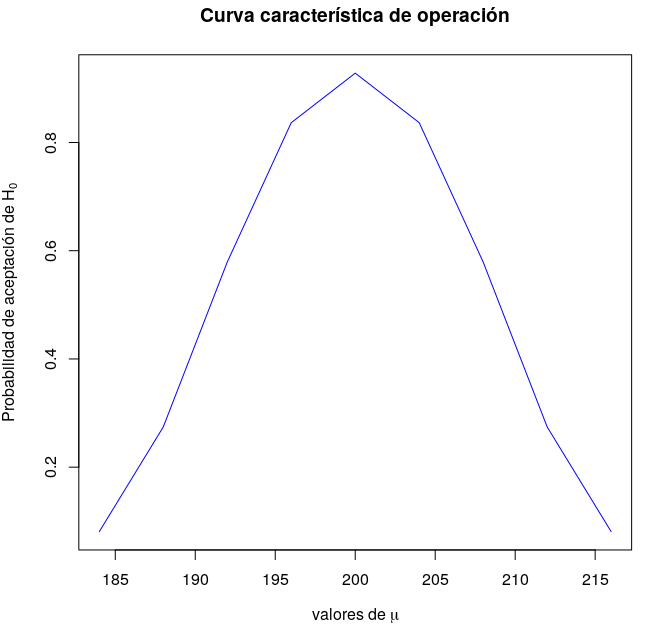
\includegraphics[scale=0.7]{Problema_18_01.png}
 \end{center}
 Aunque una gr\'afica m\'as suave se puede visualizar con los siguientes comandos:
 \begin{verbatim}
> x<-seq(184,216,0.1)
> y<-pnorm(209,mean=x,sd=5)-pnorm(191,mean=x,sd=5)
> plot(x,y,type="l",col="blue",xlab="",ylab="")
> ejexname<-expression(paste("valores de ",mu))
> ejeyname<-expression(paste("Probabilidad de aceptación de ",H[0]))
> title(main="Curva característica de operación",xlab=ejexname,ylab=ejeyname)
 \end{verbatim}
 con lo que se obtiene el siguiente gr\'afico:
 \begin{center}
  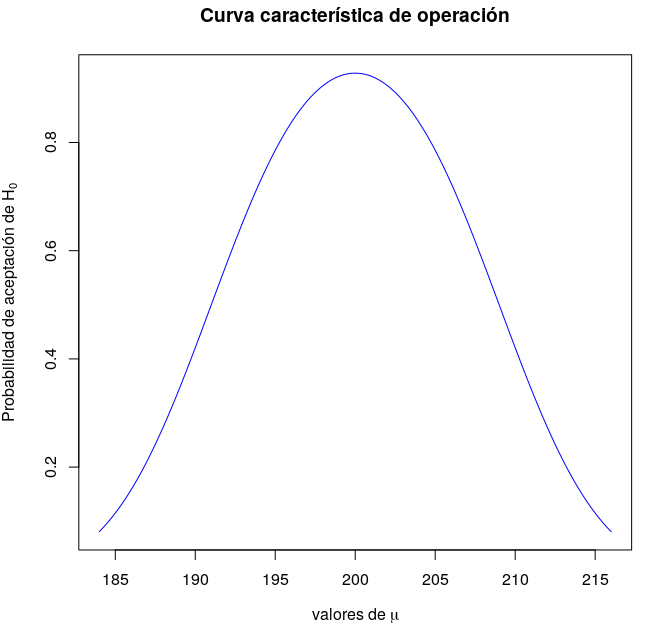
\includegraphics[scale=0.7]{Problema_18_02.png}
 \end{center}
 que es a lo que se quer\'{\i}a llegar.${}_{\blacksquare}$
\end{solucion}
